\documentclass[11pt,a4paper]{amsart}

%Fonts

\usepackage{libertine}
\usepackage{euler}
\usepackage[T1]{fontenc}

%Packages.

\usepackage{verbatim}
\usepackage{amsmath}
\usepackage{amssymb}
\usepackage{amsfonts}
\usepackage{amsthm}
\usepackage{mathrsfs}
\usepackage{tikz}
\usetikzlibrary{matrix,arrows}
\usepackage[all]{xy}
\usepackage{mathrsfs}
\usepackage{a4wide}
\usepackage{enumerate}
\usepackage{hyperref}
%\usepackage{showkeys}
\usepackage{setspace}

%Theorem styles.

\theoremstyle{plain}
\newtheorem{conj}{Conjecture}
\newtheorem{theorem}{Theorem}%[section]
\newtheorem{lemma}[theorem]{Lemma}%[section]
\newtheorem{proposition}[theorem]{Proposition}%[section]
\newtheorem{corollary}[theorem]{Corollary}%[section]
\newtheorem{claim}[theorem]{Claim}%[section]
\newtheorem{question}[theorem]{Question}
\newtheorem{conjecture}[theorem]{Conjecture}
\newtheorem*{thm}{Theorem}

\theoremstyle{definition}%[section]
\newtheorem{definition}[theorem]{Definition}%[section]
\newtheorem{example}[theorem]{Example}%[section]
\newtheorem{project}{Project}

\theoremstyle{remark}%[section]
\newtheorem{remark}[theorem]{Remark}%[section]

%Title etc.

\title{A partial action characterisation of coarse embeddability into groups and applications.} 
\date{}
\author{Martin Finn-Sell}

\begin{document}

\maketitle

\section{Introduction.}

The aim of these notes is to outline a characterisation of coarse embeddability of a metric space into a group and prove that under certain hypotheses this metric is proper. Additionally, we apply this to certain labellings of the AGS box space sequence, providing an embedding into a countable group without proper metric and conjecturing a refinement of this construction provides an embedding into a finitely generated group.

The final section is finding a home for a result about the Baum-Connes conjecture with coefficients for the Gromov monster groups that contain expanders of large girth. 

Please bear in mind these notes are very rough; I've typed them up by they avoid all the details from other papers that would need to be included to make them stand alone. Hopefully the references are complete enough. Thanks for looking at this, basically. 

\section{Partial actions and coarse embeddability.}

\begin{definition}
Let $\Gamma$ be a finitely generated discrete group and let $X$ be a (locally compact Hausdorff) topological space. A \textit{partial action} of $\Gamma$ on $X$ is a dual prehomomorphism that has the following properties:
\begin{enumerate}
\item The domain $D_{\theta_{g}^{*}\theta_{g}}$ is an open set for every $g$.
\item $\theta_{g}$ is a continuous map.
\item The union: $\bigcup_{g \in G}D_{\theta_{g}^{*}\theta_{g}}$ is $X$.
\end{enumerate}
We say that the action is \textit{transitive} if for every pair of points $(x,y) \in X^{2}$ there is a $g\in \Gamma$ such that $\theta_{g}(x)=y$ and \textit{free} if for every point, the set $\lbrace g \in \Gamma | \theta_{g}(x)=x \rbrace=\lbrace 1_{\Gamma} \rbrace$.
\end{definition}

The advantage of studying partial actions is the additional flexibility of working with partial bijections. However it is often useful to convert this data back into something tangible with regards to the group. In this manner, we introduce the globalisation; that is a space on which the group acts that extends the original partial action.

\begin{definition}
A \textit{globalisation} of a partial action $\theta: G \rightarrow I(X)$ is a space $Y$ with an injection $X \hookrightarrow Y$ and action $\tilde{\theta}$ of $G$ such that the partial action obtained from restricting the action $\tilde{\theta}$ to $X$ is equal to $\theta$. 
\end{definition}

A globalisation is minimal if it injects into any other globalisation. In \cite{MR2041539} the authors proved that for any partial action of a group $G$ there is a unique globalisation (up to equivalence of partial actions). This is defined as follows:

\begin{definition}
Let $X$ be a topological space and let $G$ be a group acting partially on $X$. Then we denote by $\Omega$ the \textit{Morita envelope} of the action of $G$ on $X$, which is constructed as follows:

Consider the space $X\times G$, equipped with the product topology. Then define $\sim$ on $X\times G$ by $(x,g)\sim (y,h)$ if and only if $x(h^{-1}g)=y$. We define $\Omega$ as the quotient of $X\times G$ by $\sim$ with the quotient topology. 

$G$ acts on $\Omega$ using right multiplication by inverses on the group factor of the equivalence classes. Clearly the map that sends $x \in X$ to $[1,x] \in \Omega$ is a topological injection. The main result of \cite{MR2041539} is that this new topological space is minimal amongst globalisations of $X$.
\end{definition}

One useful outcome of globalization of the partial action is to get an idea of the structure of the original space. Let $G_{x}$ denote the subgroup of $G$ given by the set:
\begin{equation*}
\lbrace g \in G | \theta_{g}(x) \mbox{ is defined and equal to } x \rbrace.
\end{equation*} 

\begin{theorem}\label{Thm:Free}\cite[Theorem 2.6]{MR2419858}
For a transitive partial action $\theta: G \rightarrow I(X)$ and $x_{0} \in X$ the set $G/ G_{x_{0}}$ is equivalent to the space $\Omega$ defined above.
\end{theorem}

\begin{corollary}\label{Cor:FreeTrans}
If the partial action is also assumed to be free then the minimal globalisation is given by the group $G$ itself.
\end{corollary}

Remark that given a space with a partial action that is free and transitive, we certainly get an embedding of the space into the group in question. The idea is to show that this map must be coarse. We give related ideas from coarse geometry.

\begin{definition}
Let $X$ be a set and let $\mathcal{E}$ be a collection of subsets of $X \times X$. If $\mathcal{E}$ has the following properties:
\begin{enumerate}
\item $\mathcal{E}$ is closed under finite unions;
\item $\mathcal{E}$ is closed under taking subsets;
\item $\mathcal{E}$ is closed under the induced product and inverse that comes from the groupoid product on $X \times X$.
\item $\mathcal{E}$ contains the diagonal
\end{enumerate}
Then we say $\mathcal{E}$ is a \textit{coarse structure} on $X$ and we call the elements of $\mathcal{E}$ \textit{entourages}. If in addition $\mathcal{E}$ contains all finite subsets then we say that $\mathcal{E}$ is \textit{weakly connected}.
\end{definition}

For a given family of subsets $\mathcal{S}$ of $X \times X$ we can consider the smallest coarse structure that contains $\mathcal{S}$. This is the coarse structure generated by $\mathcal{S}$. We can use this to give some examples of coarse structures.

\begin{definition}
Let $X$ be a coarse space with a coarse structure $\mathcal{E}$ and consider $\mathcal{S}$ a family of subsets of $\mathcal{E}$. We say that $\mathcal{E}$ is generated by $\mathcal{S}$ if every entourage $E \in \mathcal{E}$ is contained in a finite union of subsets of $\mathcal{S}$.
\end{definition}

\begin{example}\label{ex:MCS}
Let $X$ be a metric space. Then consider the collection $\mathcal{S}$ given by the $R$-neighbourhoods of the diagonal in $X\times X$; that is, for every $R>0$ the set:
\begin{equation*}
\Delta_{R}=\lbrace (x,y) \in X \times X | d(x,y)\leq R \rbrace
\end{equation*}
Then let $\mathcal{E}$ be the coarse structure generated by $\mathcal{S}$. This is called the \textit{metric coarse structure} on $X$. It is a uniformly locally finite proper coarse structure that is weakly connected when $X$ is a uniformly discrete bounded geometry (proper) metric space.
\end{example}

\begin{example}\label{ex:GACS}
Let $G$ be a group and let $X$ be a right $G$-set. Define:
\begin{equation*}
\Delta_{g}=\lbrace (x,x.g) | x \in X \rbrace  
\end{equation*}
We call the coarse structure generated by the family $\mathcal{S}:=\lbrace \Delta_{g} | g\in G\rbrace$ the \textit{group action coarse structure} on $X$. If $X$ is not a transitive $\Gamma$-space the group action coarse structure will not be weakly connected.
\end{example}

In the situation that $X$ admits a transitive $G$-action by translations, the group action coarse structure generates a substructure of the metric coarse structure. If additionally, each $\Delta_{R}$ is contained in finitely many $\Delta_{g}$, then the group action coarse structure will be the same as the metric coarse structure.

\begin{theorem}\label{Thm:Embedding}
If a metric space $X$ admits a free, transitive partial action of a discrete group $\Gamma$ such that for each $R>0$ there are $g_{1},...,g_{n_{R}} \in \Gamma$ such that $\Delta_{R}(X) \subseteq \bigcup_{i=1}^{n_{R}}\theta_{g_{i}}$ then the map $i$ from globalisation theorem is a coarse embedding.
\end{theorem}
\begin{proof}
Fix a proper metric on $\Gamma$, given by a length function $l$. We remark that by definition of the minimal globalisation we know that the inclusion $i$ induces an equivalence of the partial actions $\mathcal{T}_{\Gamma}|_{X}$ and $\mathcal{T}$. As both these sets generate the metric coarse structure in their respective metrics, we see that for any $R>0$: $(x,y)\in \Delta_{R}(X)=\sqcup_{i=1}^{k_{R}}t_{i}$. Set $S_{R}:=\sup \lbrace l(\overline{t_{i}}) | i=1,...,k_{R} \rbrace$. Then $(i(x),i(y))\in \Delta_{S_{R}}^{\Gamma}$. Similarly, for any pair $(i(x),i(y)) \in \Delta^{\Gamma}_{R}(i(X))=\sqcup_{j=1}^{k_{R}^{\Gamma}} g_{j}|_{i(X)}$. For each $g|_{i(X)}$ there is a unique $t_{j}\in \mathcal{T}$ such that algebraically: $(x,y)\in t_{j} \Leftrightarrow (i(x),(i(y)) \in g_{j}|_{i(X)}$. Set $S_{R}:=\sup \lbrace \vert t_{j} \vert | j=1,...,k_{R}^{\Gamma} \rbrace$. This proves that the bijection $i$ is a coarse equivalence. 
\end{proof}

\section{A strengthening of Theorem \ref{Thm:Embedding}}

Let $S$ be a semigroup and let $s \in S$. Then $u$ is said to be an \textit{inverse} for $s$ if $sus=s$ and $usu=u$. A semigroup $S$ is \textit{regular} if every element $s$ has some inverse element $u$, and \textit{inverse} if that inverse element is unique, in which case we denote it by $s^{*}$. Groups are examples of semigroups that are inverse with only a single idempotent. It is clear that in an inverse semigroup $S$ every element $ss^{*}$ is idempotent, and this classifies the structure of idempotents \cite{MR1455373}. We remark also that the idempotents of $S$ form a commutative inverse subsemigroup $E(S)$ that can be partially ordered using this multiplication: Let $e,f \in E(S)$ then:
\begin{equation*}
e \leq f \Leftrightarrow ef=e
\end{equation*}
is a partial order on $E(S)$ that extends to $S$ using:
\begin{equation*}
s \leq t \Leftrightarrow (\exists e \in E) et=s
\end{equation*}
If $s$ and $t$ are partial bijections on some set $X$ this describes precisely when $s$ is a restriction of $t$ to some subset of $dom(t)$.

This order allows us to define a more rigid and accessible class of inverse semigroup:

\begin{definition}
Let $z \in S$. We say $z$ is a zero element if $z \in E(S)$ and $zs=sz=z$. The empty partial bijection is an example of such a zero element. With this in mind we say $S$ is 0-E-unitary if $\forall e \in E\setminus 0, s \in S$ $e \leq s$ implies $s \in E$.
\end{definition}

For concrete semigroups of partial bijections this condition is equivalent to the restriction of any element never being an idempotent.

Let $S$ be a inverse semigroup. Then it is possible to define a \text{universal group} for $S$ \cite{MR2058453}, denoted by $U(S)$, to be the group generated by the elements of $S$ with relations $s\cdot t = st$ if $st \not = 0$. Clearly, there is a map $\Phi$ from $S$ to the universal group $U(S)$, given by mapping $s$ to its corresponding symbol in $U(S)$. This map is \textit{not} a homomorphism, but after adjoining a zero element to $U(S)$ does satisfy the inequality $\Phi(st) \leq \Phi(s)\Phi(t)$. Such a map is called a \textit{prehomomorphism}. 

\begin{definition}
We say $S$ is 0-F-inverse if the preimage of each group element in $U(S)$ has a maximal element within the partial order of $S$. In this case, we denote these elements by $Max(S)$, and the universal group is generated by the set $Max(S)$ with the product: $s\ast t = u$, where $u$ is the unique maximal element above $st \in S$. 

Finally, $S$ is said to be strongly $0$-F-inverse if it is $0$-F-inverse and there is some group $\Gamma$ and a $0$-restricted idempotent pure homomorphism onto $G^{0}$. In particular, this must factor though the universal group, so this amounts to asking if the map $\Phi$ is idempotent pure.
\end{definition}

In general, universal groups are hard to calculate. They play a role in determining the structure of this class of inverse monoid however \cite{MR2058453}. This class of inverse monoid is also intimately connected to partial actions of discrete groups. We need an intermediate object called the Birget-Rhodes expansion \cite{MR745358}  of a group $\Gamma$.

\begin{example}
In \cite{MR745358,MR2221438} a inverse monoid was introduced that is universal for dual prehomomorphisms from a general inverse semigroup. In the context of a group $\Gamma$ this is called the \textit{prefix expansion}; its elements are given by pairs: $(X,g)$ for $\lbrace 1,g\rbrace \subset X$, where $X$ is a finite subset of $\Gamma$. The set of such $(X,g)$ is then equipped with a product and inverse:
\begin{equation*}
(X,g)(Y,h) = (X\cup gY,gh)\mbox{ , } (X,g)^{-1}=(g^{-1}X,g^{-1})
\end{equation*}
This has maximal group homomorphic image $\Gamma$, and it has the universal property that it is the largest such inverse monoid. We denote this by $\Gamma^{Pr}$. The partial order on $\Gamma^{Pr}$ can be described by reverse inclusion, induced from reverse inclusion on finite subsets of $\Gamma$. It is F-inverse, with maximal elements: $\lbrace(\lbrace 1,g \rbrace, g):g \in \Gamma \rbrace$.
\end{example}

\begin{proposition}\label{Prop:Strongly}
Let $S = \langle \theta_{g} | g \in \Gamma \rangle$, where $\theta: \Gamma \rightarrow S$ is a partial action. If $S$ is 0-F-inverse with $Max(S) = \lbrace \theta_{g} | g \in \Gamma \rbrace$ where each nonzero $\theta_{g}$ is not idempotent when $g \not = e$ then $S$ is strongly 0-F-inverse; it has a $0$-restricted idempotent pure homomorphism onto $\Gamma$.
\end{proposition}
\begin{proof}
We build a map $\Phi$ back onto $G^{0}$. Let $m: S\setminus \lbrace 0 \rbrace \rightarrow Max(S)$ be the map that sends each non-zero $s$ to the maximal element $m(s)$ above $s$ and consider the following diagram:
\begin{equation*}
\xymatrix{
G\ar@{->}[r]^{\theta}\ar@{->}[dr]^{}  & S\ar@{->}[dr]^{\Phi}  & \\
  & G^{pr} \ar@{->}[r]^{\sigma}\ar@{->}[u]^{\overline{\theta}}  & G^{0}
}
\end{equation*}
where $G^{pr}$ is the prefix expansion of $G$. Define the map $\Phi:S \rightarrow G^{0}$ by:
\begin{equation*}
\Phi(s)=\sigma ( m ( \overline{\theta}^{-1} (m(s)))), \Phi(0)=0
\end{equation*}
For each maximal element the preimage under $\overline{\theta}$ is well defined as the map $\theta_{g}$ has the property that $\theta_{g}=\theta_{h} \Rightarrow g=h$ precisely when $\theta_{g} \not = 0 \in S$. Given the preimage is a subset of the F-inverse monoid $G^{pr}$ we know that the maximal element in the preimage is the element $(\lbrace 1,g \rbrace,g)$ for each $g \in G$, from where we can conclude that the map $\sigma$ takes this onto $g \in G$.

We now prove it is a prehomomorphism. Let $\theta_{g},\theta_{h} \in S$, then:
\begin{eqnarray*}
\Phi(\theta_{g})=\sigma ( m(\overline{\theta}^{-1}(\theta_{g}))) = \sigma ( \lbrace 1,g \rbrace, g)= g\\
\Phi(\theta_{h})=\sigma ( m(\overline{\theta}^{-1}(\theta_{h}))) = \sigma ( \lbrace 1,h \rbrace, h)= h\\
\Phi(\theta_{gh})=\sigma ( m(\overline{\theta}^{-1}(\theta_{gh}))) = \sigma ( \lbrace 1,gh \rbrace, gh)= gh
\end{eqnarray*}
Hence whenever $\theta_{g},\theta_{h}$ and $\theta_{gh}$ are defined we know that $\Phi(\theta_{g}\theta_{h})=\Phi(\theta_{g})\Phi(\theta_{h})$. They fail to be defined if:
\begin{enumerate}
\item If $\theta_{gh} = 0$ in $S$ but $\theta_{g}$ and $\theta_{h} \not = 0$ in $S$, then $0=\Phi(\theta_{g}\theta_{h})\leq \Phi(\theta_{g})\Phi(\theta_{h})$

\item If (without loss of generality) $\theta_{g}=0$ then $0=\Phi(0.\theta_{h})= 0.\Phi(\theta_{h})=0$
\end{enumerate}
So prove that the inverse monoid $S$ is strongly 0-F-inverse it is enough to prove then that the map $\Phi$ is idempotent pure, and without loss of generality it is enough to consider maps of only the maximal elements - as the dual prehomomorphism property implies that in studying any word that is non-zero we will be less than some $\theta_{g}$ for some $g \in G$.

So consider the map $\Phi$ applied to a $\theta_{g}$:
\begin{equation*}
\Phi(\theta_{g})=\sigma ( m(\overline{\theta}^{-1}(\theta_{g}))) = \sigma ( \lbrace 1,g \rbrace, g)= g
\end{equation*}

Now assume that $\Phi(\theta_{g}) = e_{G}$. Then it follows that $\sigma (m (\overline{\theta}^{-1}(\theta_{g})))=e_{G}$. As $\sigma$ is idempotent pure, it follows then that $m(\overline{\theta}^{-1}(\theta_{g}))=1$, hence for any preimage $t\in \theta^{-1}(\theta_{g})$ we know that $t \leq 1$, and by the property of being 0-E-unitary it then follows that $t \in E(G^{pr})$. Mapping this back onto $\theta_{g}$ we can conclude that $\theta_{g}$ is idempotent, but by assumption this only occurs if $g = e$.\end{proof}

\begin{corollary}
Let $S = \langle \theta_{g} | g \in \Gamma \rangle$, where $\theta: \Gamma \rightarrow S$ is a free partial action. If $S$ is 0-F-inverse with maximal elements $Max(S) = \lbrace \theta_{g} | g \in \Gamma \rbrace$ then $S$ is strongly $0$-F-inverse.\qed
\end{corollary}

\begin{definition}\label{Def:PTS}
Let $X$ be a countable set. A collection of partial bijections $\mathcal{T}$ is a called a \textit{abstract partial translation structure} for $X$ if:
\begin{enumerate}
\item $\mathcal{T}$ partitions $X\times X$.
\item $\forall t_{i}, t_{j} \in \mathcal{T}$ $\exists t_{k} \in \mathcal{T}$ we have $t_{i}t_{j} \subseteq t_{k}$ (i.e $\mathcal{T}$ is subclosed).
\item $\forall t \in \mathcal{T}$ we have $t^{*} \in \mathcal{T}$.
\item $\mathcal{T}$ has a global identity, denote this $t_{0}$.
\end{enumerate}
\end{definition}
Every abstract partial translation structure generates a coarse structure. If that coarse structure is the metric coarse structure then we just call it a \textit{partial translation structure}. 

Every abstract partial translation structure is a collection of partial bijections that contains all inverses so it generates submonoid of $I(X)$.

\begin{lemma}
The inverse monoid $S$ generated by a partial translation structure $\mathcal{T}$ is $0$-F-inverse. 
\end{lemma}
\begin{proof}
First we prove maximality of the translations. We prove that for any $s\in S \setminus \lbrace 0 \rbrace$ there exists a unique $t \in \mathcal{T}$ such that $s \leq t$. Property (2) from the Definition \ref{Def:PTS} implies that any product of elements of $\mathcal{T}$ is less than a unique $t \in \mathcal{T}$. As $\mathcal{T}$ partitions $X \times X$ we have that for any pair $t_{i},t_{j}\in \mathcal{T}$ $et_{i}=et_{j} \Leftrightarrow t_{i}=t_{j}$. 

Now we prove that $S$ is $0$-E-unitary. Let $e\in E(S)\setminus \lbrace 0 \rbrace$ and $s\in S\setminus \lbrace 0 \rbrace$. As any product of translations is included in a unique translation, it is enough to consider the case that $s$ is maximal. It follows that $e \leq s$ implies that $s$ fixes some elements of $X$. However, $\mathcal{T}$ partitions $X \times X$ and so $s \leq id_{X}$. We assumed that $s$ was maximal however, so $s = id_{X}$. Now any general word in $\mathcal{T}$ satisfies: $e \leq s \implies s \leq id_{X}$, hence $s$ is idempotent.  
\end{proof}

A partial translation structure is called \textit{strong} if the inverse monoid generated by $S$ is strongly $0$-F-inverse. The examples of partial translation structures that arise from groups are all strong.

\begin{theorem}\label{Thm:SPTSCE}
If $X$ is a discrete proper metric space with a strong partial translation structure $\mathcal{T}$ then it coarsely embeds into a countable group equipped with a proper metric.
\end{theorem}
\begin{proof}
Let $S$ be the inverse monoid generated by $\mathcal{T}$. This is strongly $0$-F-inverse by assumption; let $\Gamma$ be the universal group of $S$. We make use of this universal group by observing that $\mathcal{T}$ is a partial action of $\Gamma$ that is both free and transitive. Let $\overline{t}$ be the symbol in $\Gamma$ that arises from $t \in S$. The map $\theta: \Gamma \rightarrow I(X)$ given by $\overline{t} \mapsto t \in \mathcal{T}$. This is clearly a dual prehomomorphism and it is transitive as $\mathcal{T}$ partitions $X\times X$. Lastly it is free, as otherwise some $t \in \mathcal{T}$ must be idempotent on at least one point of $X$.

We can now globalize this action. By Corollary \ref{Cor:FreeTrans} this globalisation is $\Gamma$. We now consider the map in this instance; pick a basepoint $x_{0} \in X$. There is a unique partial translation that maps each $x$ to $x_{0}$ and we denote this by $t_{x}$. This gives rise to a subset of $\Gamma$, via the prehomomorphism that exists between $S$ and $\Gamma$ as $\mathcal{T}$ is strong. The map is injective as it is injective on the maximal elements of $S$, which is $\mathcal{T}$. To observe that this map is coarse we use Theorem \ref{Thm:Embedding}.
\end{proof}

\begin{remark}
This actually characterises coarse embeddability into groups; see Theorem 29 \cite{MR2363428}.
\end{remark}

\section{Embedding spaces of graphs into groups.}

\subsection{Partial actions from labellings.}

\begin{lemma}\label{Lem:GenPet}
Let $X$ be a finite graph. If at most $2k$ edges go into any vertex then all the edges of $X$ can be divided into $k$ classes such that at most two edges from the same class go into any vertex.\qed
\end{lemma}

Pedersen labellings allow for the construction of partial actions, they insure that the action is well defined. Certain sequences of finite graphs, such as box spaces of finitely generated residually finite groups, admit a Pedersen labellings. The partial action in this instance is an action. However, that action is certainly not free.

We introduce a few technical criteria for an edge labelling.

\begin{definition}
We say an edge labelling in a finite alphabet $A$ is \textit{Pedersen} if the partition given by the letters $a \in A$ satisfies Lemma \ref{Lem:GenPet}.
\end{definition}

It is immediate that a graph with a Pedersen labelling admits a partial action of the free group $F_{A}$. Given a sequence of finite graphs with a Pedersen labelling, the induced partial action of the free group $F_{A}$ may not be free, for instance any cycle in the $X_{i}$ will give rise to a fixed point for the word labelling that cycle.

\begin{definition}
An edge labelling of a graph $X$ is called \textit{coherent} if the label that appears on any cycle in does not appear on any proper path.
\end{definition}

Given a labelling in some finite alphabet $A$ that is both coherent and Pedersen  we can improve the partial action of $F_{A}$ to a free partial action in the following way. Consider the group $\Gamma$ given by the presentation $\langle A | \mathcal{R} \rangle$, where the set $\mathcal{R}$ consists of all the words that appear as labels of a cycle in the graph $X$. This group is a quotient of the free group $F_{A}$, which acts freely partially on $X$ via the labelling. This action is well defined due to the coherency of the labelling. We remark here that this proves the group is certainly infinite if the graph $X$ has paths of arbitrary length, and is the universal group constructed from inverse monoid associated to this partial action.

We have just proved the following:

\begin{theorem}
Given a sequence of finite graphs $\lbrace X_{i} \rbrace$ such that the space of graphs $X$ has a coherent Pedersen labelling. Then the group $\Gamma$ constructed above acts freely partially on $X$.
\end{theorem}

The action constructed above obviously generates the graph metric on $X$, but is not transitive so we do not yet have a coarse embedding of $X$ into $\Gamma$. We add the transitivity by by constructing a partial translation structure from this partial action.

\begin{proposition}\label{Prop:CheapTrick}
Given the free partial action of the discrete group $\Gamma$ on a space of graphs $X$ there is a strong partial translation structure $\mathcal{T}$ on $X$ built from the action that has universal group $\Gamma\ast F_{\infty}$.
\end{proposition}
\begin{proof}
Let $\theta: \Gamma \rightarrow I(X)$ be the partial action that generates the metric on $X$. Then define $\mathcal{T}:=\lbrace \theta_{g} | g \in \Gamma \rbrace \cup \lbrace t_{x,y} | x,y \in X\times X \rbrace$, where $t_{x,y}$ is the map defined on the singleton $x$, that sends it to the singleton $y$. Clearly now $\mathcal{T}$ satisfies the axioms of an abstract partial translation structure, and it also generates the metric coarse structure because the partial action does. 

We compute the universal group. It clearly has a quotient that is $\Gamma$, however we observe also that it is generated by $\lbrace \theta_{g} | g \in \Gamma \rbrace$ and $t_{x_{i},x_{i+1}}$ where the set of the $x_{i}$ are base points of the $X_{i}$. The only relations in the universal group are those in the $\theta_{g}$, or $t_{x,y}=\theta_{g_{i}}t_{x_{i},x_{i+k}}\theta_{g_{i+k}}$, where $g_{i},g_{i+k}$ are labels on the shortest path between $x$ to $x_{i}$ and $x_{i+k}$ to $y$ respectively. This gives a map: $\Gamma \ast F_{\infty} \rightarrow U(\mathcal{T}$ which is well defined as as the only possible ambiguity of choices in the decomposition occurs in the $g_{i}$, which are chosen based on shortest paths. If there are two shortest paths between $x$ and $x_{i}$ then we observe that they form a cycle, and hence the composites of the labels form a relation in $\Gamma$. This also proves the map is  injective. As every possible word in $U(\mathcal{T})$ can be decomposed this way, this map extends to the wanted equality: $U(\mathcal{T})=\Gamma \ast F_{\infty}$.

To see that the inverse monoid generated by $\mathcal{T}$ is strong, we observe that it is generated by a free transitive partial action of $U(\mathcal{T})$ and so it follows by Proposition \ref{Prop:Strongly}.
\end{proof}

This allows us to complete a coherent Pedersen labelling on a space of graphs into a constructible coarse embedding by adding transitivity and applying Theorem \ref{Thm:SPTSCE}

The remainder of the paper is going to be focused on constructing a coherent Pedersen labelling on a particular sequence of finite graphs with large girth.

\section{Preliminaries on large girth graphs and small cancellation sentences.}

\subsection{AGS box space.}

See the paper \cite{MR2899681}. Will fill this in as time goes on. We have certain useful numbers associated to this sequence to compile and we need to prove a small combinatorial lemma concerning the barycentric subdivisions and sizes of the edge set that have a square number of edges.

We will be considering the following seed graph:

\begin{center}
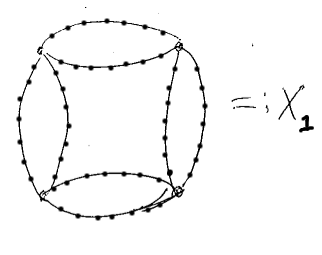
\includegraphics[scale=0.6]{seed.png}
\end{center}

As a sequence of covers it is possible to describe the number of edges in the compliment of a spanning tree of each $X_{i}$; thereby computing the degree of the deck transformation group of the covering $X_{i+1}$. We give the formula:

\begin{equation*}
d_{i}=(d_{i-1}-1)2^{d_{i-1}) + 1
\end{equation*} 
Where $d_{0}=2$, then $d_{1}=5$. 


We call the shortest cycles in the graph $X_{i}$, which have length $2^{i+3}$, cycles of \textit{type I}. Otherwise, a cycle will be \textit{type II}. Denote by $c_{I,i}$ a cycle with the same length as a type I cycle in $X_{i}$ (so  $2^{i+3}$). 

Clearly, the edge set of the graph decomposes into the edge sets of some number of cycles of length $\vert c_{I} \vert$. 

\subsection{A set of small cancellation words of Erchler-Osin.}

For this section, we need an early section of \cite{MR2136537}, mostly concerned again with certain numerical 
values that have significance in this work. 

Explain the construction at a later date.

It is enough to know here that they construct a family of words, for every $n$, that have length $n^{2}$ and satisfy small cancellation criteria $\lambda_{i}$, where the $\lambda_{i} \rightarrow 0$ in $i$. The construction passes through an auxillary set, which contains words of length $\lfloor \sqrt{n} \rfloor$ \cite{MR2136537}. 

The overall set is denoted $T$, which is the union of the sets $T(n)$ for every $n$. 

In order to label cycles using these words, we observe that we require  $\lfloor \sqrt{2^{i+3}} \rfloor$ to be an integer; we choose the graphs where $i+3$ is even, and so $i$ is odd. We remark that technical constraints also require us to choose some $i_{0} \in \mathbb{N}$ and consider the infinite tail: 
\begin{equation*}
X_{>i_{0},odd}= \sqcup_{\substack{i>i_{0}\\ i \mbox{ odd}}}X_{i}
\end{equation*}

\section{Barycentric subdivision.}

Let $\lbrace Z_{i} \rbrace$ be a sequence of finite graphs with uniformly bounded degree. Then we construct a new sequence of graphs by barycentric subdividing each edge into $k_{i}$ new edges. This graph, if $k_{i}$ is bounded, is coarsely equivalent to the original sequence and so if we give as input a sequence of large girth, the new space will not have property A. We will outline this in the next section.

\subsection{Bounded barycentric subdivsion.}

As the graphs $X_{i}$ have only even vertex degrees they each admit an Euler cycle. Additionally, every edge belongs to a unique cycle of type I, and so there is a bijection $E(X_{i}) = \sqcup_{j=1}^{l} c_{i,j}$, where $l$ is the number of cycles of type I. Each of these cycles has the same length, $\vert c_{i,j} \vert = k2^{i}$, where $k$ is the number of barycentric subdivisions applied to the original seed graph $Y$.

By picking an initial vertex $v_{j}$ in each cycle $c_{i,j}$ it is possible to label $c_{i,j}$ using a word in $T(2^{i+3})$. This labelling then gives us a edge labelling $L$ of the graph $X_{i}$. Doing this for every $i>i_{0}$ for some calculable $i_{0}$ gives us a labelling of the space of graphs $X_{>i_{0}}$, which we denote by $\mathcal{L}_{0}$. This will not in general be Pedersen, so we remedy this by adjusting the $X_{i}$.

Given a finite graph $X$ with vertices of degree $2$ and $4$ (as we have above) and a labelling $L$, it is possible to construct a new graph $Y$ by replacing each vertex of degree 4 by two vertices joined by an edge. Now the maximal degree in $Y$ is $3$. We perform this construction on the entire sequence $X_{i}$ from above to get a sequence $Y_{i}$. We remark that this is in essence constructed from the disjoint union of the short cycle representatives of each $X_{i}$ by adding an edge between any two vertices that would be glued together in $X_{i}$. 

\begin{center}
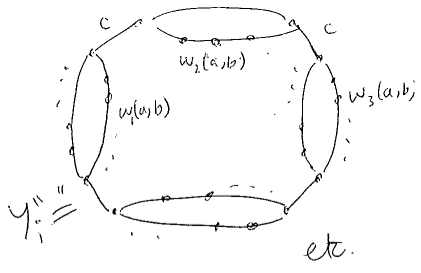
\includegraphics[scale=0.6]{Y.png}
\end{center}

The spaces of graphs constructed from the $\lbrace X_{i} \rbrace$ and $\lbrace Y_{i} \rbrace$ are coarsely equivalent. Using the technique above, we can construct labelling on the $Y_{i}$ where each type I cycle is labelled by a word in $T(2^{i+3})$ and the new edges are labelled by a new letter $c$. Denote this new labelling by $\mathcal{L}_{1}$. The following lemma is now clear:

\begin{lemma}\label{lem:modpedersen}
The labelling $\mathcal{L}_{1}$ is Pedersen. 
\end{lemma}

Now the following also holds $\mathcal{L}_{1}$:

\begin{lemma}\label{lem:shortcoherent}
Let $c_{i}$ be a type I cycle in $Y_{i}$ and let $p$ be any proper subpath of a type $I$ cycle in $Y_{\geq i+1}$. Then the label of $p$ contains no more than $\lambda_{i}$ of the label of $c_{i}$. 
\end{lemma}
\begin{proof}
Let $p$ be as described, and let $c_{j}$ be the type $I$ cycle that contains $p$ and denote by $w_{c_{i}}$ and $w_{c_{j}}$ the labels of the cycles $c_{i}$ and $c_{j}$. Lastly, denote by $w$ the subword of $w_{c_{j}}$ that labels $p$. Assume for a contradiction that there is a common subword $w^{'}$ of $w$ and $w_{c_{i}}$ that satisfies $\vert w\vert \geq\lambda_{i} \vert w_{c_{i}} \vert$. This subword is also a subword of$w_{c_{j}}$ and by the small cancellation condition on words in $\cup_{\geq i} T(2^{i+3})$ we know that any common subword of $w_{c_{i}}$ and $w_{c_{j}}$ has length at most $\lambda_{i} \vert w_{c_{i}} \vert$. 
\end{proof}

Lemma \ref{lem:shortcoherent} implies that the labelling is coherent for cycles of type $I$. This leaves a proof for cycles of type II. Let $p$ be a proper path and let $c$ be a cycle in $Y$. Let $i$ be the smallest natural number such that $p$ and $c$ are contained in some $X_{\geq i}$. If the labelling $w_{p}$ matches the labelling $w_{c}$ then we know it can contain at most $\lambda_{i}\vert c_{i,I} \vert$ of the label of any type I cycle in $X_{i}$. In fact, this means that $w_{p}=\prod_{j=1}^{k}b_{j}c$, where $\vert b_{j} \vert < \lambda_{i}\vert c_{i,I} \vert$. We call these subwords $b_{j}$ \textit{blocks}.

We get the following estimate on $\vert w_{p} \vert = \sum_{j=1}^{k} (\vert b_{j} \vert +1) < k(\lambda_{i}\vert c_{i,I} \vert +1)$, which in turn implies that the number of blocks is greater than $1\backslash \lambda_{i}$.

And this is the best I can do to fix this situation.

To be clear, the consequences of this working out as coherent are the following: 

\begin{theorem}
The group $\Gamma$ constructed using the partial action induced by the labelling $\mathcal{L}_{1}$ does not have property A.
\end{theorem}
\begin{proof}
The sequence of graphs $X_{>i_{0},odd}$ admits a coherent Pedersen labelling $\tilde{L}$ that induces a free partial action of $\Gamma$. $\Gamma$ is also the universal group of $S(L)$, the inverse monoid generated by the labelling. We extend this labelling to a strong partial translation structure $\mathcal{T}$ using Proposition \ref{Prop:CheapTrick} and then apply Theorem \ref{Thm:SPTSCE} to get a coarse embedding into the universal group $U(S(\mathcal{T}))$. By Theorem \ref{Thm:SPTSCE} this universal group is isomorphic to $\Gamma \ast F_{\infty}$. As a consequence this does not have property A in any proper metric, from where we deduce that $\Gamma$ itself does not have property A by permanence properties \cite{EG-permanence} and Theorem 4.3.9 of \cite{MR2562146}. 
\end{proof}

\begin{conjecture}
The labelling $\mathcal{L}_{1}$ is coherent.
\end{conjecture}

\subsection{What about graphical small cancellation?}

Graphical small cancellation conditions introduced throughly in \cite{DG-graphical} give rise to coherent Pedersen labellings;  consider the contrapositive. Remark then that one could consider the goal of constructing a graphical small cancellation labelling explicitly to utilise these results. In fact, however, there is a view that these currently weaker conditions.

\subsection{An alternative approach to the problem of coherence.}

Here we define a new method of understanding a graph with a cycle decomposition as we have constructed above. Let the space $Z_{i}$ denote the graph given by the disjoint union of $c_{i,j}$, where each $c_{i,j}$ is isomorphic to $c_{I,i}$ and $j=1,...,l_{i}$, where $l_{i}$ is the number of type $I$ cycles in $X_{i}$. 

Then we can label $Z_{i}$ (in a coherent way) using the words from $T(2^{i+3})$, as above. To get $X_{i}$ from $Z_{i}$ requires some kind of equivalence relation on vertices; we represent this a different way using an inverse monoid as follows. Define $S$ using labelling in $a,b$, by considering the labels as partial maps on $Z_{i}$ in the usual way. Now, this means that certain words in $T(2^{i+3})$ are idempotent in $S$.

\begin{center}
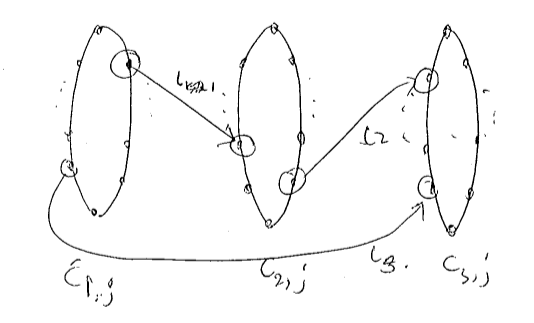
\includegraphics[scale=0.6]{invsemigraph.png}
\end{center}

To turn this into something built from a partial action on $X_{i}$, we add a new letter $e_{i,m}$ for each of the $m$ pairs of vertices that should be glued together (or connected by an edge in $Y_{i}$, for instance) and let $e_{i,m}$ act by mapping the single initial vertex of this edge to the terminal one and be defined nowhere else. Now clearly, the semigroup generated by $S$ and these new maps corresponding the missing connections, will describe a labelling of $Y_{i}$. It is also clear that applying this construction for every $i$ labelling of $Y$. This labelling will be in the alphabet $B:=\lbrace a,b e_{1,0},...,e_{i,m},... \rbrace$, which is countable. It is clearly both Pedersen and coherent (good), but also will not give a coarse embedding into a group with a proper metric as each $e_{i,m}$ would need to have a bounded length, but cannot possibly in the universal group with any proper metric (bad). Denote this semigroup by $S_{\infty}$.

So we can imagine a process of fixing this in one step: define a partial bijection $c$ that does all the $e_{i,m}$ simultaenously. This gives us back the semigroup generated by the labelling $\mathcal{L}_{2}$. It is of course not clear that this is coherent. But we can also proceed by first gluing $e_{1,0}$ to $e_{1,1}$, and then performing some induction. This would give us a very large commuting diagram of quotients of $S_{\infty}$, which will have a direct limit $S(\mathcal{L}_{2})$. The issue is whether or not the quotient semigroups are strongly 0-F-inverse; whether or not is is possible to slowly replace finitely many $e_{i,m}$ with single grouped partial bijections $e_{m^{'}}$.

This rephrasing still gets me nowhere, but it illustrates that the problem is hard. And tells me that there is a countable group with a stupid metric that coarsely contains the AGS space... this was probably known before but it is quite neat. :)

\bibliographystyle{plain}
\bibliography{/home/mfinnse/Documents/Work/NoteonUEG/ref.bib}


\end{document}